\subsection{bpmsimulation/digitise.c File Reference}
\label{digitise_8c}\index{bpmsimulation/digitise.c@{bpmsimulation/digitise.c}}


\subsubsection{Detailed Description}


Definition in file {\bf digitise.c}.

{\tt \#include $<$bpm/bpm\_\-messages.h$>$}\par
{\tt \#include $<$bpm/bpm\_\-simulation.h$>$}\par
{\tt \#include $<$bpm/bpm\_\-rf.h$>$}\par
{\tt \#include $<$bpm/bpm\_\-nr.h$>$}\par
{\tt \#include $<$bpm/bpm\_\-wf.h$>$}\par


Include dependency graph for digitise.c:\nopagebreak
\begin{figure}[H]
\begin{center}
\leavevmode
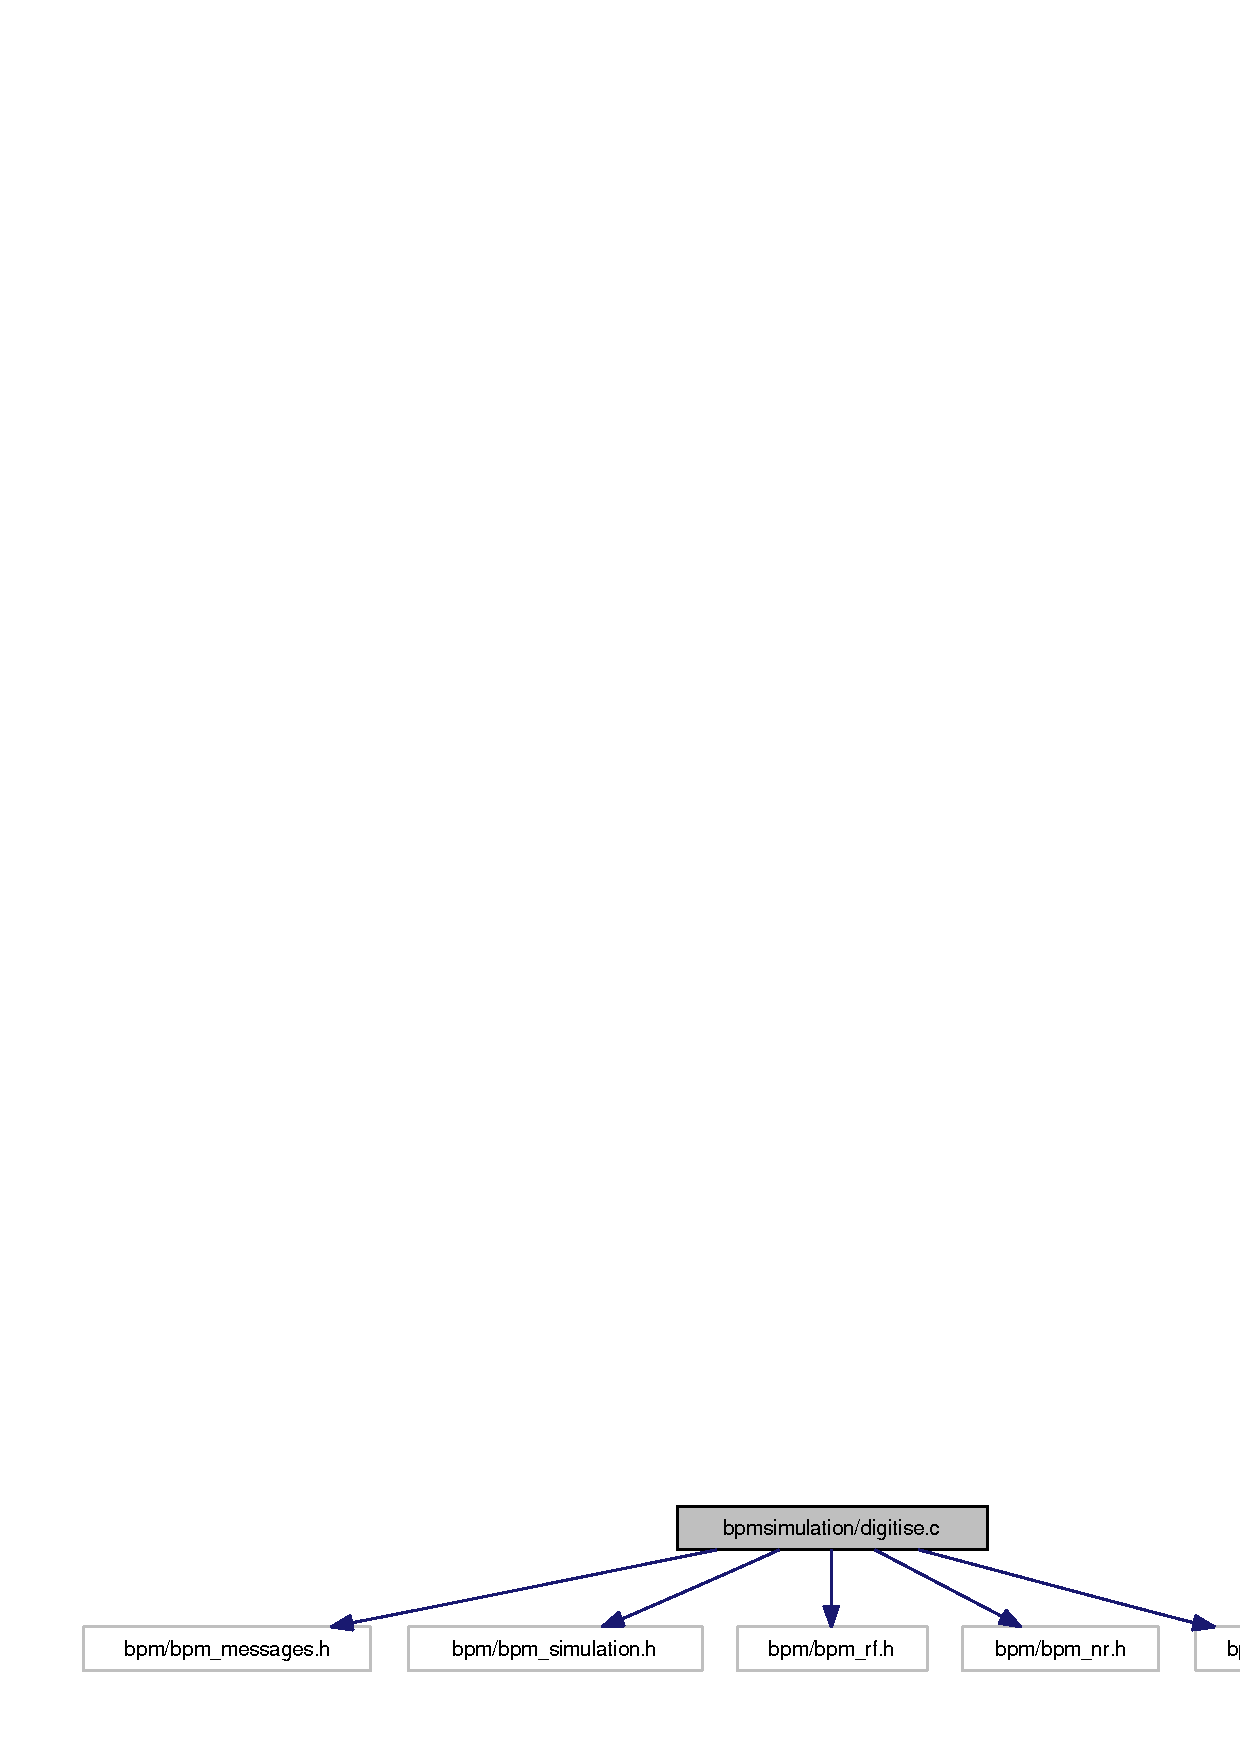
\includegraphics[width=336pt]{digitise_8c__incl}
\end{center}
\end{figure}
\subsubsection*{Functions}
\begin{CompactItemize}
\item 
int {\bf digitise} ({\bf doublewf\_\-t} $\ast$IF, int nbits, double range\_\-min, double range\_\-max, double clock\_\-jitter, double digi\_\-noise, unsigned int ipmode, {\bf intwf\_\-t} $\ast$wf)
\end{CompactItemize}
